\documentclass[t]{beamer}

% Load general definitions
% Preamble file - general definitions, package loading, etc.

%=================================
% Load packages
\usepackage{amssymb,amsmath}
\usepackage{graphicx}
\usepackage{url}
\usepackage{tikz}
\usetikzlibrary{mindmap,trees,arrows}
\usepackage{fancyvrb}
\usepackage[portuguese]{babel} 
\usepackage[utf8]{inputenc}
\usepackage{subfigure}
\usepackage{times}
\usepackage[T1]{fontenc}
\usepackage{cancel}
\usepackage{color}
\usepackage{listings}
\usepackage[document]{ragged2e}

%=================================
% Set mode
\mode<presentation>
{
	\usetheme{Madrid}
	\usecolortheme{structure}
	\useoutertheme{infolines}
	\setbeamercovered{invisible}
}

% Get rid of nav bar
\beamertemplatenavigationsymbolsempty

% Insert frame number at bottom of the page.
\usefoottemplate{\hfil\tiny{\color{black!90}\insertframenumber}} 

%=================================
% Define new commands

\newcommand\Real{{\mathbb{R}}}
%\newcommand{\vi}{\vspace{0.6\baselineskip}}
%\newcommand{\goodgap}{\hspace{\subfigtopskip}\hspace{\subfigbottomskip}}


% Equation environments
\newcommand{\beq}{\begin{equation}}
\newcommand{\eq}{\end{equation}}
\newcommand{\beqs}{\begin{equation*}}
\newcommand{\eqs}{\end{equation*}}
\newcommand{\beqn}{\begin{eqnarray}}
\newcommand{\eqn}{\end{eqnarray}}
% Bold variables
\newcommand{\mbf}[1]{\ensuremath{\mathbf{#1}}}
% Itemization
\newcommand{\bitem}{\begin{itemize}}
\newcommand{\eitem}{\end{itemize}}
\newcommand{\spitem}{\vskip 1em\item}
\newcommand{\bitems}{\begin{itemize}\item}
\newcommand{\benums}{\begin{enumerate}\item}
\newcommand{\eenum}{\end{enumerate}}
% color blocks
\newenvironment{colorblock}[2]{%
\setbeamercolor{block title}{#2}
\begin{block}{#1}}{\end{block}}
% Vertical spacing
\newcommand{\vone}{\vskip 1em}
\newcommand{\vhalf}{\vskip .5em}
% Frame environments
\newenvironment{ftst}[3][t]{%
\begin{frame}{environment=ftst,#1}
\frametitle{#2}
\framesubtitle{#3}}{\end{frame}}
\newenvironment{ftstf}[2]{
\begin{frame}[fragile,environment=ftstf]
\frametitle{#1}
\framesubtitle{#2}}{\end{frame}}
% colors
\definecolor{MyGray}{rgb}{0.5,0.5,0.5}
\definecolor{MyDBGray}{rgb}{0.1,0.1,0.4}
\definecolor{darkgreen}{rgb}{0,0.4,0}
\definecolor{black}{rgb}{0,0,0}
\def\defn#1{{\color{red} #1}}
% Footnote
\renewcommand{\thefootnote}{\alph{footnote}}
% Relaxed footnotes
\newcommand{\lfr}[1]{\let\thefootnote\relax\footnote{\tiny #1}}
% Verbatim environment - using FANCYVRB package
\DefineVerbatimEnvironment%
{rcode}{Verbatim}
{fontsize=\scriptsize}
% Verbatim environment - using LISTINGS package
%\lstnewenvironment{rcode} {\lstset{	language = R,
%									basicstyle = \scriptsize\ttfamily,
%									showspaces = false,
%									showstringspaces = false,
%									showtabs = false,
%									keywordstyle = \color{black}\bfseries,
%									commentstyle = \color{darkgreen},
%									numbers = none,
%									otherkeywords={	<-,
%													ggplot,
%													geom_boxplot,
%													facet_grid,
%													shapiro.test,
%													fligner.test,
%													glht,
%													with},
%									deletekeywords={data,
%													model,
%													residuals,
%													c,
%													axis,
%													default,
%													labels,
%													qq.text}}}%
%{}

% Specific definitions
\title[]{Metodologia Científica}
\subtitle[]{Preparação do texto}
\author[]{Patrícia Lucas\\{\footnotesize }}
\institute{Bacharelado em Sistemas de Informação \\ IFNMG  - Campus Salinas}
\date{\scriptsize Salinas\\Junho 2021}

\begin{document}

% cover page
\setbeamertemplate{footline}{}
\begin{frame}

\begin{center}
\includegraphics[width=.15\textwidth]{}
\end{center}
  \titlepage
  \begin{tikzpicture}[remember picture,overlay]
  \node[anchor=south east,xshift=-5pt,yshift=5pt] at (current page.south east) {\tiny Versão 1.2021};
  \node[anchor=south west,yshift=0pt] at (current page.south west) {
\includegraphics[width=.25\textwidth]{Logos/salinas_horizontal_jpg.jpg}};
  \end{tikzpicture}  
\end{frame}

% Main slides

\begin{ftst}{Referência}{Preparação do texto}

\justifying
\begin{figure}
    \centering
    
\includegraphics[scale=0.35]{Figuras/ref2.jpg}
\end{figure}

Gastel, Barbara; Day, Robert A. How to Write and Publish a Scientific Paper. Califórnia: Greenwood, 2016.

\end{ftst}

%=====


\begin{ftst}{O título}{Preparação do texto}
\justifying
A importância do título:
\vone
\begin{itemize}
    \item O título é simplesmente a referência principal ao trabalho.
    \item  É a chave pela qual o trabalho será referenciado, deve refletir o
    conteúdo do trabalho, bem como ser claro, curto e correto.
    \item  O título é um nome, não uma frase, deve ser original e não
    necessariamente a primeira coisa a se escrever no trabalho.
\end{itemize}


\end{ftst}

%=====

\begin{ftst}{O resumo}{Preparação do texto}
\justifying
\begin{itemize}
    \item Um resumo deve ser visto como uma versão em miniatura do artigo.
    \vone
    \item Um resumo bem preparado permite que os leitores identifiquem o conteúdo básico de um documento com rapidez e precisão, determinem sua relevância para seus interesses e, assim, decidam se precisam ler o documento em sua totalidade.
    \vone
    \item O resumo não deve exceder o comprimento especificado pela revista (normalmente, 250 palavras).
\end{itemize}

\end{ftst}

%=====

\begin{ftst}{O resumo}{Preparação do texto}
\justifying
\begin{itemize}
    \item Normalmente, o resumo deve ser digitado como um único parágrafo.
    \vone
    \item Alguns periódicos, entretanto, executam resumos “estruturados” que consistem em alguns parágrafos breves, cada um precedido por um subtítulo padronizado.
\end{itemize}

\end{ftst}

%=====

\begin{ftst}{O resumo}{Preparação do texto}
\justifying
\begin{figure}
    \centering
    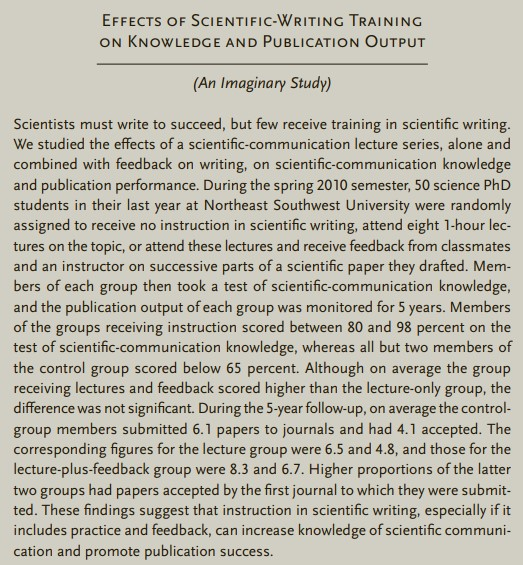
\includegraphics[scale=0.5]{Figuras/resumo1.jpg}
\end{figure}

\end{ftst}

%=====

\begin{ftst}{O resumo}{Preparação do texto}
\justifying
\begin{figure}
    \centering
    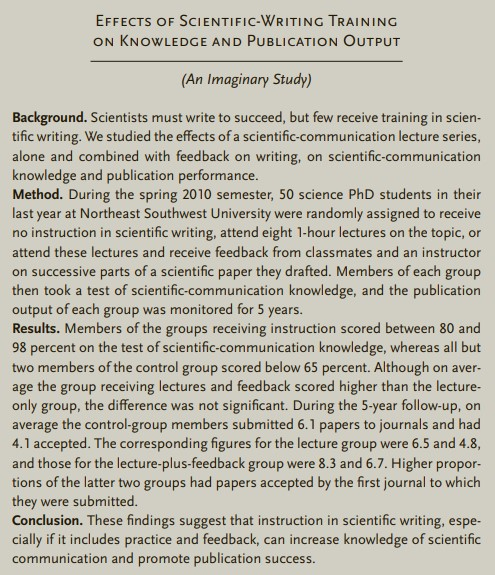
\includegraphics[scale=0.5]{Figuras/resumo2.jpg}
\end{figure}

\end{ftst}

%=====

\begin{ftst}{O resumo}{Preparação do texto}
\justifying
\begin{itemize}
    \item A maior parte ou todo o resumo deve ser escrito no pretérito porque se refere ao trabalho realizado.
    \vone
    \item O resumo nunca deve fornecer qualquer informação ou conclusão que não esteja declarada no artigo.
    \vone
    \item A literatura não deve ser citada no resumo (exceto em casos raros, como modificação de um método publicado anteriormente).
    \vone
    \item Da mesma forma, normalmente o resumo não deve incluir ou referir-se a tabelas e figuras.
\end{itemize}

\end{ftst}

%=====

\begin{ftst}{O resumo}{Preparação do texto}
\justifying
Sugestão de como escrever um resumo:
\vone
\begin{itemize}
    \item[1. ] Contexto geral e específico.
    \item[2. ] Questão/problema sendo investigado.
    \item[3. ] Estado da arte: por que precisa de uma solução nova/melhor?
    \item[4. ] Solução: nome da proposta, metodologia básica sem detalhes, quais características respondem as questões iniciais.
    \item[5. ] Interpretação dos resultados, conclusões.
\end{itemize}


\end{ftst}

%=====

\begin{ftst}{O resumo}{Preparação do texto}
\justifying
Exemplo:
\vone
\small
\textbf{CONTEXTO:} \textit{"A Web é abundante em páginas que armazenam dados de forma implícita."}
\vone
\textbf{PROBLEMA:} \textit{"Em muitos casos, estes dados estão presentes em textos semiestruturados sem a presença de delimitadores explícitos e organizados em uma estrutura também implícita."}
\vone
\textbf{SOLUÇÃO:} \textit{"Neste artigo é apresentada uma nova abordagem para extração em textos semi-estruturados baseada em Modelos de Markov Ocultos (Hidden Markov Models - HMM)."}



\end{ftst}

%=====

\begin{ftst}{O resumo}{Preparação do texto}
\justifying
Exemplo:
\vone
\small
\textbf{ESTADO-DA-ARTE e MÉTODO PROPOSTO:} \textit{"Ao contrário de outros trabalhos baseados em HMM, nossa abordagem dá ênfase à extração de metadados além dos dados propriamente ditos. Esta abordagem consiste no uso de uma estrutura aninhada de HMMs, onde um HMM principal identifica os atributos no texto e HMMs internos, um para cada atributo, identificam os dados e metadados. Os HMMs são gerados a partir de um treinamento com uma fração de amostras da base a ser extraída."}
\vone
\textbf{RESULTADOS:} \textit{"Os experimentos com anúncios de
classificados retirados da Web mostram que o processo de
extração alcançáveis de qualidade acima de 0,97 com a medida F,
mesmo se esta fração de treinamento é pequena."}

\end{ftst}

%=====

\begin{ftst}{A introdução}{Preparação do texto}
\justifying
\small
\begin{itemize}
    \item Um artigo \textbf{NÃO} é um livro de suspense no qual o leitor só descobre o que está realmente acontecendo no capítulo final. 
    \item O leitor deve estar ciente do que acontece desde o início, desde a introdução.
    \item Deve fornecer uma declaração de forma breve e clara do seu propósito ao escrever o artigo.
    \item Escolha as referências com cuidado para fornecer as informações básicas mais importantes.
    \item Grande parte da introdução deve ser escrita no tempo presente porque você está se referindo principalmente ao seu problema e ao conhecimento relacionado a ele no início do seu trabalho.
    
\end{itemize}
\end{ftst}

%=====

\begin{ftst}{A introdução}{Preparação do texto}
\justifying
Sugestão de como escrever uma introdução (um ou dois parágrafos por item):
\small
\vone
\begin{itemize}
    \item[1.] Contexto, motivação.
    \item[2.] O problema em questão.
    \item[3.] Trabalhos anteriores relacionados (limitações).
    \item[4.] Contribuições.
    \item[5.] Organização das seções do trabalho.
\end{itemize}
\end{ftst}

%=====

\begin{ftst}{A introdução}{Preparação do texto}
\justifying
Exemplo de \textbf{contexto}:
\small
\vone
\textit{"A computação distribuída era uma fazenda de servidores autocontidos e co-localizados. Hoje, os aplicativos são cada vez mais implantados em recursos de terceiros hospedados na Internet. De fato, a rápida disseminação de protocolos e padrões abertos como a Web 2.0 alimentou uma explosão de serviços compostos que fazem script de componentes de terceiros para fornecer um serviço sofisticado [27, 29]. Esses serviços especializados são apenas o começo: os principais aplicativos corporativos e de consumo estão cada vez mais sendo entregues no modelo software-a-serviço [9]. Por exemplo, Google Documents, Groove Office e Windows Live são os primeiros exemplos de aplicativos de desktop fornecidos em um ambiente hospedado, e representam o início de uma tendência muito maior."}
\end{ftst}

%=====

\begin{ftst}{A introdução}{Preparação do texto}
\justifying
Exemplo de \textbf{problema}:
\small
\vone
\textit{"Uma das principais barreiras para mover aplicativos tradicionais para a nuvem, entretanto, é a perda de controle de custos [17]. No modelo de serviços baseados em nuvem, a recuperação de custos normalmente é realizada por meio de preços medidos. Na verdade, o EC2 da Amazon cobra incrementalmente por gigabyte de tráfego consumido [3]. Limitar o consumo de recursos globais em um ambiente distribuído, no entanto, apresenta um desafio técnico significativo. Idealmente, os provedores de recursos não exigiriam serviços para especificar as demandas de recursos de cada componente distribuído a priori. Essa medição e modelagem de baixa granularidade podem ser desafiadoras para serviços em rápida evolução. Em vez disso, eles devem fornecer um preço fixo para um uso global agregado e permitir que os serviços consumam recursos dinamicamente em vários locais, sujeito ao limite agregado especificado."}
\end{ftst}

%=====

\begin{ftst}{A introdução}{Preparação do texto}
\justifying
Exemplo de \textbf{trabalhos anteriores relacionados (limitações)}:
\small
\vone
\textit{"Como resposta a tal requisito, alguns trabalhos têm enfocado a questão do suporte a versões [2,4,9,13,23,27]. Entre esses, Golendziner propõe o Modelo de Versões: uma extensão aplicável a modelos de dados orientado a objetos ...[9].}"
\end{ftst}

%=====

\begin{ftst}{A introdução}{Preparação do texto}
\justifying
Exemplo de \textbf{contribuições}:
\small
\vone
"\textit{Considerando o contexto atual, esse trabalho propõe...}"
\vone
\vone
Exemplo de \textbf{organização}:
\small
\vone
“\textit{O restante deste trabalho está organizado da seguinte maneira. A seção 2 apresenta alguns conceitos básicos e discute trabalhos relacionados. A seção 3 detalha o modelo proposto. A seção 4 apresenta um estudo comparativo através de experimentos, enquanto a seção 5 conclui o trabalho.}"
\end{ftst}

%=====

\begin{ftst}{Materiais e métodos/metodologia}{Preparação do texto}
\justifying
\begin{itemize}
    \item A maior parte desta seção deve ser escrita no pretérito.
    \vone
    \item O objetivo principal da seção de materiais e métodos é descrever (e, se necessário, defender) o projeto experimental e, em seguida, fornecer detalhes suficientes para os experimentos possa ser repetido.
    \vone
    \item A seção de materiais e métodos geralmente tem subtítulos.
    \vone
    \item Seja preciso. Os métodos são semelhantes às receitas dos livros de receitas. Se uma mistura de reação foi aquecida, forneça a temperatura. Perguntas como "como" e "quanto" devem ser respondidas com precisão pelo autor e não deixada para o revisor ou o leitor decifrar.
\end{itemize}

\end{ftst}

%=====

\begin{ftst}{Resultados}{Preparação do texto}
\justifying
\begin{itemize}
    \item Agora chegamos ao cerne do artigo.
    \vone
    \item Como você apresenta os dados? Uma simples transferência de dados do "caderno de laboratório" para o texto dificilmente será suficiente. No texto você deve apresentar dados representativos em vez de dados repetitivos infinitos.
    \vone
    \item Embora a seção de resultados seja a parte mais importante, geralmente é a mais curta, especialmente se for precedida por uma seção de materiais e métodos bem escrita e seguida por uma discussão bem escrita.
    \vone
    \item Os resultados precisam ser declarados de forma clara e simples, porque são os resultados que constituem o novo conhecimento com o qual você está contribuindo para o mundo.
\end{itemize}

\end{ftst}

%=====

\begin{ftst}{Resultados}{Preparação do texto}
\justifying
\begin{itemize}
    \item Como lidar com números: se um ou apenas alguns valores forem apresentados, eles devem ser tratados de forma descritiva no texto. Os valores repetitivos devem ser fornecidos em tabelas ou gráficos.
    \vone
    \item Evite redundâncias: se os resultados são apresentados em uma tabela, por exemplo, não precisa ser descrito no texto.
    \vone
    \item Não seja prolixo ao citar figuras e tabelas. Evite expressões como: "\textit{Está claramente mostrado na Tabela 1 que o Algoritmo X apresentou desempenho melhor que o Algoritmo Y.}" Use: "\textit{O Algoritmo X apresentou desempenho melhor que o Algoritmo Y (Tabela 1)}".
\end{itemize}

\end{ftst}

%=====

\begin{ftst}{Discussão}{Preparação do texto}
\justifying
\begin{itemize}
    \item Relacionamentos entre os fatos e resultados observados.
    \vone
    \item Princípios, relações, generalizações mostradas nos Experimentos. 
    \vone
    \item Aponte quaisquer exceções ou falta de correlação e defina os pontos não resolvidos. Nunca tome a alternativa de alto risco de tentar encobrir ou falsificar dados que não se encaixam perfeitamente.
    \vone
    \item Mostrar que resultados e interpretações concordam (ou contrastam) com trabalhos previamente publicados.
    \vone
    \item Implicações teóricas e possíveis aplicações práticas.
\end{itemize}

\end{ftst}

%=====

\begin{ftst}{Conclusão}{Preparação do texto}
\justifying
\begin{itemize}
    \item Exponha suas conclusões o mais claramente possível.
    \vone
    \item Resuma suas evidências para cada conclusão  (não assuma que o leitor é super capaz de juntar todos os pontos sozinho).
    \vone
    \item Certifique-se de que a conclusão responda ao que a introdução perguntou.
    \vone
    \item Exemplo: uma conclusão bem estruturada pode primeiro reafirmar as principais descobertas, depois discutir como elas se relacionam com as descobertas de pesquisas anteriores, depois observar as implicações e aplicações e, talvez, identificar questões não respondidas adequadas para pesquisas futuras.
\end{itemize}

\end{ftst}

\end{document}